\chapter{Desenvolvimento do modelo OLAP}
\label{cap:DesenvolvimentoDoModeloOLAP}
%-------------------------------------------------------
% descrever como foi feito o levantamento dos residuos mais interesantes. 
%  Explicar que a lista dos mais presentes foi comparada com uma lista originalmente desenvolvida por um especialista de dominio. 
%  Encontrou se casos que estavam e nao estavam na lista, os que nao apareciam na lista constituem de residuos que se ficam ˜proximos”ao sitio de ligação, mas que na realidade estão fora do sítio.
% descrever como  adicionar novas dimensoes baseadas em novos residuos
%-------------------------------------------------------

Para possibilitar a construção do modelo OLAP, primeiramente foi necessário identificar e definir as questões de negócio que seriam relevantes sob o ponto de vista do especialista de domínio. Em virtude disso, o levantamento destes dados foi feito por meio de entrevistas com os especialistas do LABIO.

A Tabela \ref{tab:questaoNegocio} descreve as questões de negócio que foram identificadas como sendo mais relevantes para execução de análise de experimentos de docagem realizados no LABIO. 

\begin{table}[h]
\caption{Questões de negócio identificadas pelos especialistas com maior relevância para análise de experimentos de docagem}
\label{tab:questaoNegocio}
\centering
\begin{tabular}{@{}ll@{}}
\toprule
\textbf{ } & \multicolumn{1}{c}{\textbf{Questões de maior relevância para a análise de docagem}}		\\ \midrule
\textbf{1.} & Associar um grupo para cada conformação;													\\
\textbf{2.} & Identificar o comportamento das conformações baseado nas métricas de FEB e RMSD;			\\
\textbf{3.} & Identificar conformações/grupos que possuem o maior número de contatos com os ligantes;	\\
\textbf{4.} & Com base no item 3, identificar quais são os resíduos mais importantes;					\\
\textbf{5.} & Com base no item 3, identificar quais grupos possuem melhores valores de FEB e RMSD.		\\ \bottomrule
\end{tabular}
\end{table}

\section{Identificação de métricas}
\label{sec:IdentificacaoDeMetricas}

Durante as entrevistas realizadas, pode-se perceber que informações baseadas nas métricas de FEB e RMSD possuíam grande relevância para responder as questões de negócio. Entretanto foi necessário definir certas propriedades e limitações de valores para adequar os cálculos às necessidades do negócio. Dessa maneira, todas as definições citadas nesta seção foram estabelecidas em conjunto com os especialistas de domínio do LABIO, para que os resultados apresentados pudessem representar a realidade.

O cálculo da FEB é um dos métodos utilizados pelos softwares de docagem que permite avaliar a interação receptor-ligante. Quanto menor for o resultado deste cálculo, mais favorável é a ligação estabelecida. Portanto, o valor estimado da FEB é utilizado como uma das métricas do modelo.

Na maioria dos experimentos, os melhores resultados de FEB são valores negativos. Portanto, qualquer conformação que apresente valores de FEB positivos não foram levados em consideração. Dessa maneira evita-se que os resultados positivos venham a interferir em uma análise futura dos valores agregados de um experimento. 

O cálculo do RMSD é utilizado para obter a distância média entre os átomos. Nos experimentos de docagem, este cálculo é feito para comparar o posicionamento inicial do ligante, geralmente estipulada pelo especialista de domínio, com o posicionamento final após a execução da docagem. Neste caso, o RMSD é considerado como uma métrica para a modelagem.

Tanto a FEB quando o RMSD dão uma visão para o especialista de quão satisfatório foi o processo de docagem para uma determinada iteração. Enquanto a FEB mede a qualidade da docagem no aspecto termodinâmico da questão, o RMSD tem como natureza avaliar geometricamente como estão dispostas as moléculas do resíduo e do ligante.

Além disso, para ser possível responder ao item 3 da Tabela \ref{tab:questaoNegocio}, foi necessário incluir uma métrica para contabilizar o número de contatos entre o ligante e um resíduo da molécula receptora. 

Um contato pode ser identificado pelo cálculo da medida em {\AA}ngstr\"om ({\AA}) entre os átomos do resíduo do receptor e do ligante. Ou seja, para cada resíduo do receptor \emph{R} é calculada a distância Euclidiana entre todos seus átomos e os átomos de um ligante \emph{L}. Sendo $R=(r_{x},r_{y},r_{z})$ representando as coordenadas dos átomos dos resíduos do receptor, e $L=(l_{x},l_{y},l_{z})$ representando as coordenadas dos átomos do ligante, o cálculo da distância se dá pela equação \ref{eqt:distEuclid}.

\begin{equation}
\label{eqt:distEuclid}
	d(R,L)=\sqrt{(r_{x}-l_{x})^{2}+(r_{y}-l_{y})^{2}+(r_{z}-l_{z})^{2}}
\end{equation}

Em suma, para cada snapshot devem ser calculadas todas as coodernadas do receptor com todas as coordenadas de cada ligante, neste caso para o TCL e para o ETH. Entretanto, de todas as distâncias calculadas para um resíduo, apenas a menor delas deve ser considerada. 

A Figura \ref{fig:PIFvsGLY} ilustra este conceito, apresentando como exemplo as distâncias entre os átomos do ligante PIF (cor preto) e do resíduo GLY95 (cor cinza) do receptor InhA. Para todas as distâncias calculadas, a menor delas é de 2.72 {\AA} \cite{KARANADUNOSM09}.

\begin{figure}[h]
	\center
	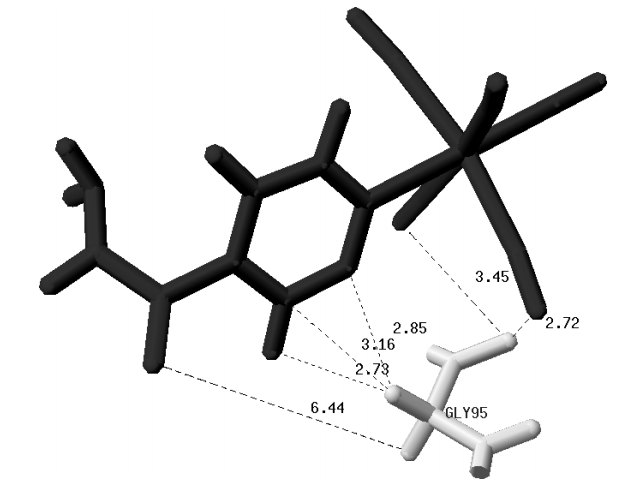
\includegraphics[scale=0.5]{images/distEucli.png}
	\caption{Cálculo das distâncias atômicas entre o ligante PIF (cor preta) e o resíduo GLY95 (cor cinza) do receptor InhA \cite{MAC10}.}
	\label{fig:PIFvsGLY}
\end{figure} 

\section{Identificação dos resíduos relevantes}

Um dos pontos mais importantes para responder aos questionamentos dos especialistas de domínio e fundamental para composição das dimensões, consiste em definir os resíduos mais relevantes para os experimentos de docagem envolvedo os ligantes TCL e ETH com o receptor InhA. 

A enzima InhA é composta de 268 resíduos, e o processo de identificação dos mais importantes leva em consideração o número de contatos estabelecidos entre os átomos do resíduo e o ligante. No \emph{dataset} que foi resultado do processo de simulação de docagem, cada átomo do resíduo está representado por uma tripla, contendo a sua localização espacial nos eixos \emph{x, y }e \emph{z}.

De acordo com o especialista de domínio, a interação entre um átomo do resíduo e o ligante só deve ser considerada como contato quando a distância entre ambos seja entre 2{\AA} e 4{\AA}. Valores inferiores a 2{\AA} são descartados por serem considerados uma sobreposição, enquanto valores superiores a 4{\AA} indicam que não foi estabelecido contato. 

Desta forma, para se obter os valores de todo o conjunto presente no \emph{dataset} foi calculado a distância Euclidiana tridimensional dos átomos através da equação \ref{eqt:distEuclid}, conforme descrito na seção \ref{sec:IdentificacaoDeMetricas}. Porém, o cálculo foi desconsiderado para todos os átomos de hidrogênio, pois estes devem ser tratados de outra forma.

Portanto, a relevância de um resíduo para um experimento de docagem aumenta em função do número de contatos estabelecidos entre seus átomos e o ligante. As regras de classificação de relevância de um resíduo podem ser sumarizadas da seguinte forma:

\begin{enumerate}
	\item São considerados contatos somente as distâncias entre 2 e 4 {\AA}ngstr\"ons.
	\item Distâncias inferiores a 2 {\AA}ngstr\"ons são desconsideradas.
	\item Átomos de hidrogênio são descartados.
	\item Quanto maior for o número de contatos estabelecidos de um resíduo, mais relevante ele se torna para o experimento.
\end{enumerate}

Além disso, um outro artefato foi utilizado para auxiliar na identificação de resíduos relevantes. Baseado em análises e estudos de experimentos anteriores utilizando a InhA como molécula receptora, um especialista de domínio elaborou uma lista dos 52 principais resíduos que possuem relevância para os experimentos de docagem baseados no mesmo cenário. A Tabela \ref{tab:listaOsmar} lista os resíduos representados pela sua sigla e seu número de ordem na enzima.

\begin{table}[h]
\caption{Lista elaborada pelo especialista de domínio com os principais resíduos para experimentos de docagem utilizando a enzima InhA.}
\label{tab:listaOsmar}
\centering
\begin{tabular}{@{}lllllll@{}}
GLY\_13	&	PHE\_40 &	PHE\_96	&	PHE\_148 &	PRO\_191 &	ILE\_201 &	GLU\_209 		\\
ILE\_14	&	LEU\_62 &	MET\_97	&	PRO\_155 &	ILE\_193 &	VAL\_202 &	ALA\_210 		\\
ILE\_15	&	ASP\_63 &	GLN\_99	&	ALA\_156 &	THR\_195 &	GLY\_203 &	ILE\_214 		\\
THR\_16	&	VAL\_64 &	MET\_102 &	TYR\_157 &	LEU\_196 &	GLY\_204 &	LEU\_217 		\\
SER\_18	&	GLN\_65 &	GLY\_103 &	MET\_160 &	ALA\_197 &	ALA\_205 &					\\
SER\_19	&	SER\_93 &	ILE\_121 &	LYS\_164 &	MET\_198 &	LEU\_206 &					\\
ILE\_20	&	ILE\_94	&	MET\_146 &	ALA\_190 &	SER\_199 &	GLY\_207 &					\\
ALA\_21 &	GLY\_95	&	ASP\_147 &	GLY\_191 &	ALA\_200 &	GLU\_208 &					\\ 
\end{tabular}
\end{table}

%----------------------
%  TO DO: REFERENCIAR ALGORITMO ---------------------------------------
%----------------------
Definido este cenário, foram executados os algoritmos descritos em \ref{alg:CalculoDistancia} para o cálculo das distâncias e sumarização dos dados. Então, após a execução foi possível obter uma listagem de 15 resíduos com maior número de contatos que eram comuns para os experimentos de docagem envolvendo ambos ligantes TCL e ETH. A Tabela \ref{tab:listaProvavelRelevantes} lista os resíduos obtidos pelo algoritmo, que estão representados pela sua sigla e seu número de ordem na enzima.

\begin{table}[h]
\caption{Resíduos identificados pelo algoritmo de classificação por relevância.}
\label{tab:listaProvavelRelevantes}
\centering
\begin{tabular}{@{}lll@{}}
ILE\_15  & ASP\_149 & MET\_160 \\
SER\_19  & ARG\_152 & ILE\_193 \\
ILE\_94  & ALA\_153 & THR\_195 \\
GLY\_95  & MET\_154 & MET\_198 \\
PHE\_148 & TYR\_157 & TRP\_221 \\
\end{tabular}
\end{table}

Com posse destes dados, os resíduos resultantes (apresentados na Tabela \ref{tab:listaRelevantes}) foram comparados com a lista feita pelo especialista de domínio (apresentados na Tabela \ref{tab:listaOsmar}) a fim de identificar os elementos que eram comuns aos dois grupos. 

Os resíduos do conjunto obtido foram plotados pelos especialistas de domínio do LABIO e estão ilustrados pela Figura \ref{fig:PlotResiduos}. Dos 15 resíduos identificados pelo algoritmo, 10 deles estão presentes na lista do especialista de domínio e foram classificados como sendo relevantes para os experimentos de docagem. Os 5 resíduos que não estavam presentes na lista do especialista foram identificados como casos onde a proteína apresentou ligações fora da cavidade do substrato e, por este motivo, não foram considerados como sendo relevantes.

\begin{figure}[h]
        \center
        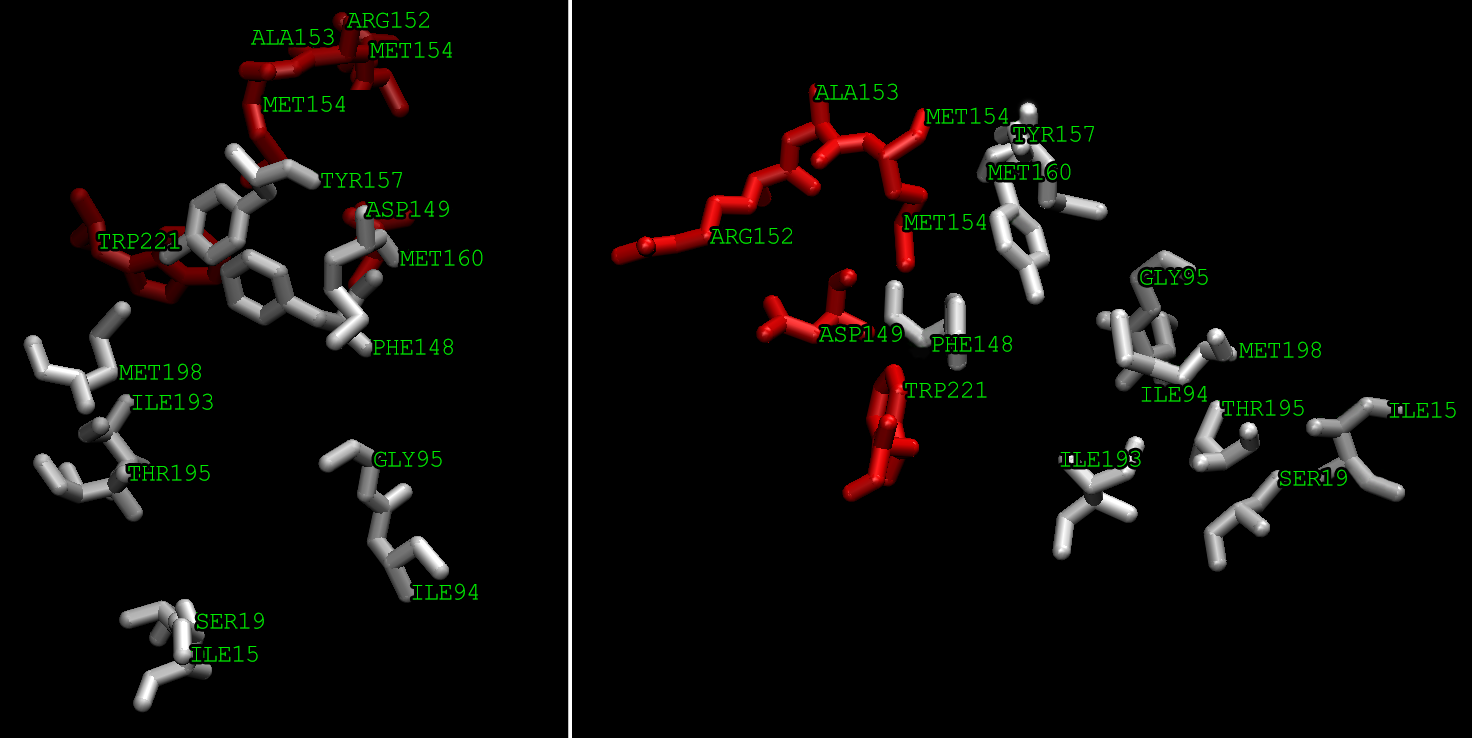
\includegraphics[width=10cm]{images/avaliacao_Residuos_nomes.png}
        \label{fig:PlotResiduos}
        \caption{Plotagem dos 15 resíduos identificados pelo algoritmo de classificação por relevância. A cor cinza representa os resíduos que são relevantes e aparecem na listagem do especialista de domínio, já os resíduos que estão em vermelho não estão presentes na lista.}
\end{figure}

Por fim, com base nestas comparações e nos experimentos realizados foi possível elencar os 10 principais resíduos mais relevantes para responder às questões de negócio. O conjunto final está listado na Tabela

\begin{table}[h]
\caption{Conjunto final de resíduos relevantes para experimentos de docagem molecular considerando como receptor a enzima da InhA e ligantes TCL e ETH.}
\label{tab:listaProvavelRelevantes}
\centering
\begin{tabular}{@{}ll@{}}
\toprule
\multicolumn{1}{c}{Resíduo} & \multicolumn{1}{c}{Nome} \\ \midrule
SER\_19                     & Serine                   \\
ILE\_15                     & Isoleucine               \\
ILE\_94                     & Isoleucine               \\
GLY\_95                     & Glycine                  \\
PHE\_148                    & Phenylalanine            \\
TYR\_157                    & Tyrosine                 \\
MET\_160                    & Methionine               \\
ILE\_193                    & Isoleucine               \\
THR\_195                    & Threonine                \\
MET\_198                    & Methionine               \\ \bottomrule
\end{tabular}
\end{table}

\section{Scripts para preparação dos dados}
\label{sec:ScriptsParaPreparacaoDosDados}

Com objetivo de automatizar o processo de preparação dos dados de simulações de docagem molecular, foram criados dois scripts utilizando as linguagens Python e Bash. O primeiro script é responsável pela sumarização dos dados resultante da simulação para posteriormente alimentar o modelo OLAP com os dados já organizados. O segundo script foi criado para manipular as colunas de um arquivo CSV contendo o resultado dos processos de docagem.

Através da distância euclidiana ($d(P, Q)= \sqrt{(x - a)^{2} +(y - b)^{2} + (z - c)^{2}}$), faz-se um filtro para obtenção das ligações mais estáveis, enquanto as ligações que apresentam valores ruins, consideradas instáveis, são descartadas.

Os dados de entrada no primeiro script de carga recebem três parâmetros. O primeiro parâmetro é um arquivo texto contendo a lista de resíduos, o segundo é um arquivo texto contendo a lista de ligantes e o terceiro é o arquivo delimitado por vírgula (CSV) contendo o resultado da simulação dos processos de docagem molecular. Após a execução deste script, tem-se como resultado os dados sumarizados e organizados, prontos para alimentar o modelo OLAP. O segundo script é responsável por excluir ou manter determinadas colunas dos arquivos CSV. Ele recebe como primeiro parâmetro uma lista de colunas separadas por vírgula, o segundo parâmetro prove as opções para excluir (-x) ou manter apenas (-m) as linhas e o terceiro é o arquivo CSV a ser manipulado.

O procedimento de execução destas rotinas pode ser definido na seguinte sequência:

\begin{enumerate}
    \item Remoção de espaços em branco do arquivo contendo o processo de simulação da docagem. 
    \item Criação das listas de resíduos e ligantes levando em consideração o arquivo com a simulação.
    \item Execução do script de manipulação do arquivo de simulação de docagem para separar os resíduos NAH e o ligante TCL, conforme determinação do especialista de domínio.
    \item Execução do script para avaliação dos melhores resultados.
    \item Sumarização dos resultados.
\end{enumerate}

% Algoritmos

\renewcommand{\algorithmicfor}{\textbf{para}}
\renewcommand{\algorithmicif}{\textbf{se}}
\renewcommand{\algorithmicthen}{\textbf{então}}
\renewcommand{\algorithmicelse}{\textbf{senão}}
\renewcommand{\algorithmicendif}{\textbf{fim se}}
\renewcommand{\algorithmicendfor}{\textbf{fim para}}
\renewcommand{\algorithmicdo}{\textbf{faça}}

\floatname{algorithm}{Algoritmo}
\begin{algorithm}[H]
\caption{Algoritmo para cálculo da distância}
\label{alg:CalculoDistancia}
{\fontsize{10}{10}\selectfont
\begin{algorithmic}[1]
	\STATE Seja R uma lista de resíduos
	\STATE Seja L uma lista de ligantes
	\STATE Seja D a base de dados dos resultados da simulação de docagem molecular
	\STATE Seja r um resíduo de R
	\STATE Seja l um ligante de L
	\STATE Seja d um \emph{snapshot} da conformação da base D
	\FOR{cada d em D}
		\FOR{cada r em R}
			\FOR{cada l em L faça}
			\IF{r não conter átomo de hidrogênio}
			\STATE Distância $\gets \sqrt{(x - a)^{2} +(y - b)^{2} + (z - c)^{2}}$ 
			\ENDIF
			\IF{Distância menor que 4}
				\IF{Distância menor ou igual a 2}
				\STATE Gravar na saída d, r, l, distancia, classificação menor que 2
				\ELSE
				\STATE Gravar na saída d, r, l, distancia, classificação entre 2 e 4
				\ENDIF
			\ENDIF
			\ENDFOR
		\ENDFOR
	\ENDFOR
\end{algorithmic}
}
\end{algorithm}

\floatname{algorithm}{Algoritmo}
\begin{algorithm}[H]
\caption{Algoritmo para manipulação da base de dados da simulação de docagem molecular}
\label{alg:ajustaColunaDocking}
{\fontsize{10}{10}\selectfont
\begin{algorithmic}[1]
	\STATE Seja C a lista com o nome das colunas
	\STATE Seja D a base de dados dos resultados da simulação de docagem molecular
	\STATE Seja c uma coluna em C
	\STATE Seja d uma linha em D
	\STATE Seja M o modo de operação da execução
	\IF{M for igual a manter as colunas em C}
		\FOR{cada d em D}
			\FOR{cada c em C}
			\STATE Grave apenas c na saída
			\ENDFOR
		\ENDFOR
	\ENDIF
	\IF{M for igual a excluir as colunas em C}
		\FOR{cada d em D}
			\FOR{cada c em C}
			\STATE Remove apenas c na saída
			\ENDFOR
		\ENDFOR
	\ENDIF
\end{algorithmic}
}
\end{algorithm}

\floatname{algorithm}{Algoritmo}
\begin{algorithm}[H]
\caption{Algoritmo para popular os dados na dimensão tempo}
\label{alg:criaDadosDIMTempo}
{\fontsize{10}{10}\selectfont
\begin{algorithmic}[1]
	\STATE Seja P um valor inteiro maior que 1
	\STATE Seja L uma lista de valores
	\STATE Seja c um contador
	\FOR{iteração em P}
		\STATE Incrementa mais um em c
		\IF{c igual a 1000}
			\STATE Armazena o valor de P em L
			\STATE Grave o comando de inserção baseado em L
			\STATE Esvazie L
			\STATE Atribua zero em c
		\ELSE
			\STATE Armazena valor de P em L
		\ENDIF
	\ENDFOR
	\IF{L não estiver vazia}
		\STATE Grave o comando de inserção baseado em L
	\ENDIF
\end{algorithmic}
}
\end{algorithm}

\floatname{algorithm}{Algoritmo}
\begin{algorithm}[H]
\caption{Algoritmo para popular os dados na fato}
\label{ciraDadosFato}
{\fontsize{10}{10}\selectfont
\begin{algorithmic}[1]
	\STATE Seja L uma lista de ligantes
	\STATE Seja l um ligante em L
	\STATE Seja G uma lista de grupos
	\STATE Seja g um grupo em G
	\STATE Seja M uma lista de modelos dinâmicos
	\STATE Seja m um modelo dinâmico em M
	\STATE Seja E uma lista de experimentos
	\STATE Seja e um experimento em E
	\STATE Seja R uma lista de resíduos mais importantes
	\STATE Seja r um resíduo em R
	\STATE Seja S uma lista de numero de contato dos resíduos
	\STATE Seja s o numero de um contato em S
	\STATE Seja D a base de dados dos resultados da simulação de docagem molecular
	\STATE Seja d uma conformação em D
	\STATE Seja a um agrupamento de d
	\STATE Seja C uma lista de comandos para inserção
	\FOR{cada l em L}
		\STATE Grave o comando de inserção baseado em l
	\ENDFOR
        \FOR{cada g em G}
		\STATE Grave o comando de inserção baseado em g
        \ENDFOR
        \FOR{cada m em M}
		\STATE Grave o comando de inserção baseado em m
        \ENDFOR
        \FOR{cada e em E}
		\STATE Grave o comando de inserção baseado em e
        \ENDFOR
	\FOR{cada r em R}
		\STATE Grave o comando de inserção baseado em r
	\ENDFOR
	\FOR{cada d em D}
		\STATE Grave a em C
		\FOR{cada l em L}
			\FOR{cada s em S}
				\STATE Gravar o valor de s em C para a composição baseando em d, l e r
			\ENDFOR
			\IF{FEB de d for positiva}
				\STATE Gravar 0 para FEB de d em C
			\ELSE
				\STATE Gravar FEB de d em C
			\ENDIF
			\STATE Gravar RMSD de d em C
			\STATE Gravar o comando de inserção baseado em C
		\ENDFOR
	\ENDFOR
\end{algorithmic}
}
\end{algorithm}

%-------------------
% TO DO:  mostrar tabela de exemplo do resultado de saída do script.
%-------------------

\section{Dimensões}
	mostrar hierarquias de dimensoes
	
\section{Construção do modelo no Analisys Services}
	exibir a tabela pivotante com os valores medios (feb,rmsd)
